% PAKETE UND DOKUMENTKONFIGURATION
\documentclass[11pt, a4paper]{article}

% Encoding für Umlaute
\usepackage[utf8]{inputenc}
\usepackage[T1]{fontenc}

% Silbentrennung
\usepackage[ngerman]{babel}

% erweiterte Matheumgebungen und Formelnummer mit Sectionnummer
\usepackage{amsmath}
\numberwithin{equation}{section}

% Braket Notation
\usepackage{braket}
\usepackage{isotope}
\usepackage[version=3]{mhchem}

% zusätzliche mathematische Schriftarten
\usepackage{amsfonts}

% verschiedene mathematische Symbole
\usepackage{amssymb}

% Einheiten setzen z.B. \SI{10}{\kilo\gram\meter\per\second\squared}
% Fehler: \SI{10 +- 0,2e-4}{\metre}
\usepackage{siunitx}
\sisetup{
  output-decimal-marker={,},
  separate-uncertainty
}

% Einheitendefinitionen
\DeclareSIUnit{\skt}{Skt.}
\DeclareSIUnit{\gauss}{G}
\DeclareSIUnit{\division}{div.}

% Operatordefinitionen
\DeclareMathOperator{\erf}{erf}

% Randbreiten
\usepackage[left=3.5cm,right=3.5cm,top=3cm,bottom=3cm,twoside]{geometry}

% Bilder einfügen
\usepackage{graphicx}

% Verweise innerhalb des Dokuments
\usepackage{hyperref}
\hypersetup{
	colorlinks = true,
	allcolors = {black}
}

% bessere Tabellenlayouts
\usepackage{booktabs}
\usepackage{multirow}
\usepackage{multicol}

% Seitenlayout (Kopfzeile)
\usepackage{fancyhdr}

% Float Barriers
\usepackage{placeins}

% Pakete für gedrehte Subfigures
\usepackage{caption}
\usepackage{subcaption}
\usepackage{rotating}

% Paket für textumflossene Abbildungen und Tabellen
\usepackage{wrapfig}

\usepackage{float}

% Caption-Setup
\captionsetup{font={small}}
\renewcommand{\thefigure}{\thesection.\arabic{figure}}
\renewcommand{\thesubfigure}{\alph{subfigure}}
\renewcommand{\thetable}{\thesection.\arabic{table}}
\renewcommand{\thesubtable}{\alph{subtable}}

% Manuelle Silbentrennung
\hyphenation{Sig-nal-ver-hal-ten Szin-til-la-tions-de-tek-tors}

% Tiefe des Inhaltsverzeichnisses (Level: 1 sections, 2 subsections,
% 3 subsubsections)
\setcounter{tocdepth}{3}

% FANCYHDR SETUP
\pagestyle{fancy}
\fancyhead[EL,OR]{\thepage}
\fancyhead[ER]{\leftmark}
\fancyhead[OL]{\rightmark}
\setlength{\headheight}{13.6pt}

\renewcommand{\sectionmark}[1]{
\markboth{\thesection{} #1}{\thesection{} #1}
}
\renewcommand{\subsectionmark}[1]{
\markright{\thesubsection{} #1}
}

\newcommand{\ptt}{Peak-to-Total-Verhältnis}
\newcommand{\co}{\isotope[60]{Co}}
\newcommand{\cs}{\isotope[137]{Cs}}
\newcommand{\eu}{\isotope[152]{Eu}}

% DOKUMENTINFORMATIONEN
\title{P529 \\ Dosimetrie und Abschirmung}

\author{Christopher Deutsch\footnote{christopher.deutsch@uni-bonn.de} \and Christian Bespin\footnote{christian.bespin@uni-bonn.de}}

\date{\today}

\begin{document}

\begin{titlepage}

\maketitle

% DURCHFÜHRUNGSDATUM UND TUTOR
\begin{center}
\begin{tabular}{l r}
Durchführung: & 4./5. Mai 2015 \\
Gruppe: & $\alpha$ 6 \\
Tutor: & Marcus Gruener
\end{tabular}
\end{center}

% ZUSAMMENFASSUNG
\begin{abstract}
\noindent
\end{abstract}

\end{titlepage}

% INHALTSVERZEICHNIS
\tableofcontents
% Neue Seite nach TOC
\newpage

% INHALT VERSUCHSPROTOKOLL

\section{Einführung}

\section{Theorie}
\subsection{Röntgenstrahlung}
Als Röntgenstrahlung wird der Teil des elektromagnetischen Spektrums mit Photon-Energien zwischen \SI{100}{\electronvolt} und \SI{100}{\kilo\electronvolt} bezeichnet, wobei diese Grenzen nicht scharf sind und deshalb oft hinsichtlich der Strahlungsquelle eine Einordnung vollzogen wird.

\subsubsection{Erzeugung}
\label{sec:röntgenerzeugung}
Es gibt zwei typische Erzeugungsmethoden von Röntgenstrahlung, welche auf dem Beschuss eines \emph{Targets} mit einem hochenergetischen Elektronenstrahl bestehen.
Die beiden Strahlungsarten, welche in der Praxis oft zusammen auftreten, sind:
\begin{itemize}
	\item \textbf{Bremsstrahlung:} Die bei der Streuung der geladenen Elektronen an den Kernen des Targets vollzogene Geschwindigkeitsänderung des Elektrons, führt zur Emission eines Photons.
	Das so entstandene Spektrum ist kontinuierlich, wobei die maximale Photonenenergie gegeben ist durch die kinetische Energie der einfallenden Elektronen, welche durch deren Beschleunigungsspannung $U$ gegeben ist.
	Überträgt das Elektron seine gesamte Energie auf ein einzelnes Photon:
	\begin{align}
	&E_\mathrm{kin. e^-} = h \cdot \nu_\mathrm{max} = \frac{hc}{\lambda_\mathrm{min}}
	\end{align}
	so ist diese Grenze gegeben durch das \textbf{Duane-Hunt-Gesetz}
	\begin{align}
	\lambda_\mathrm{min} = \frac{h c}{e U}
	\end{align}
	Eine Quelle für reine Bremsstrahlung sind Synchrotronstrahlungsquellen.
	
	\item \textbf{charakteristische Strahlung:} Die einfallende hochenergetische Elektronenstrahlung ionisiert ein Elektron der inneren Schale eines Targetatoms.
	Dadurch entsteht ein freier Zustand, welcher durch ein Elektron einer weiter äußeren Schale eingenommen werden kann.
	Durch den Übergang wird ein Photon emittiert, dessen Energie gleich der Energiedifferenz der beiden Zustände ist.
	Aufgrund dieser Abhängigkeit von der elektronisches Struktur des Targetatoms, ist das emittierte, diskrete Spektrum charakteristisch für das verwendete (Target)-Material.
	Außerdem weist das emittierte Spektrum die Aufspaltung der Energieniveaus aufgrund von Fein- und Hyperfeinstruktur auf.
\end{itemize}
In der Praxis treten beide Effekte bei der Erzeugung von Röntgenstrahlen in sogenannten Röntgenröhren auf, wie in Abbildung \ref{fig:spektrum} zu sehen ist.
\begin{figure}[ht]
	\centering
	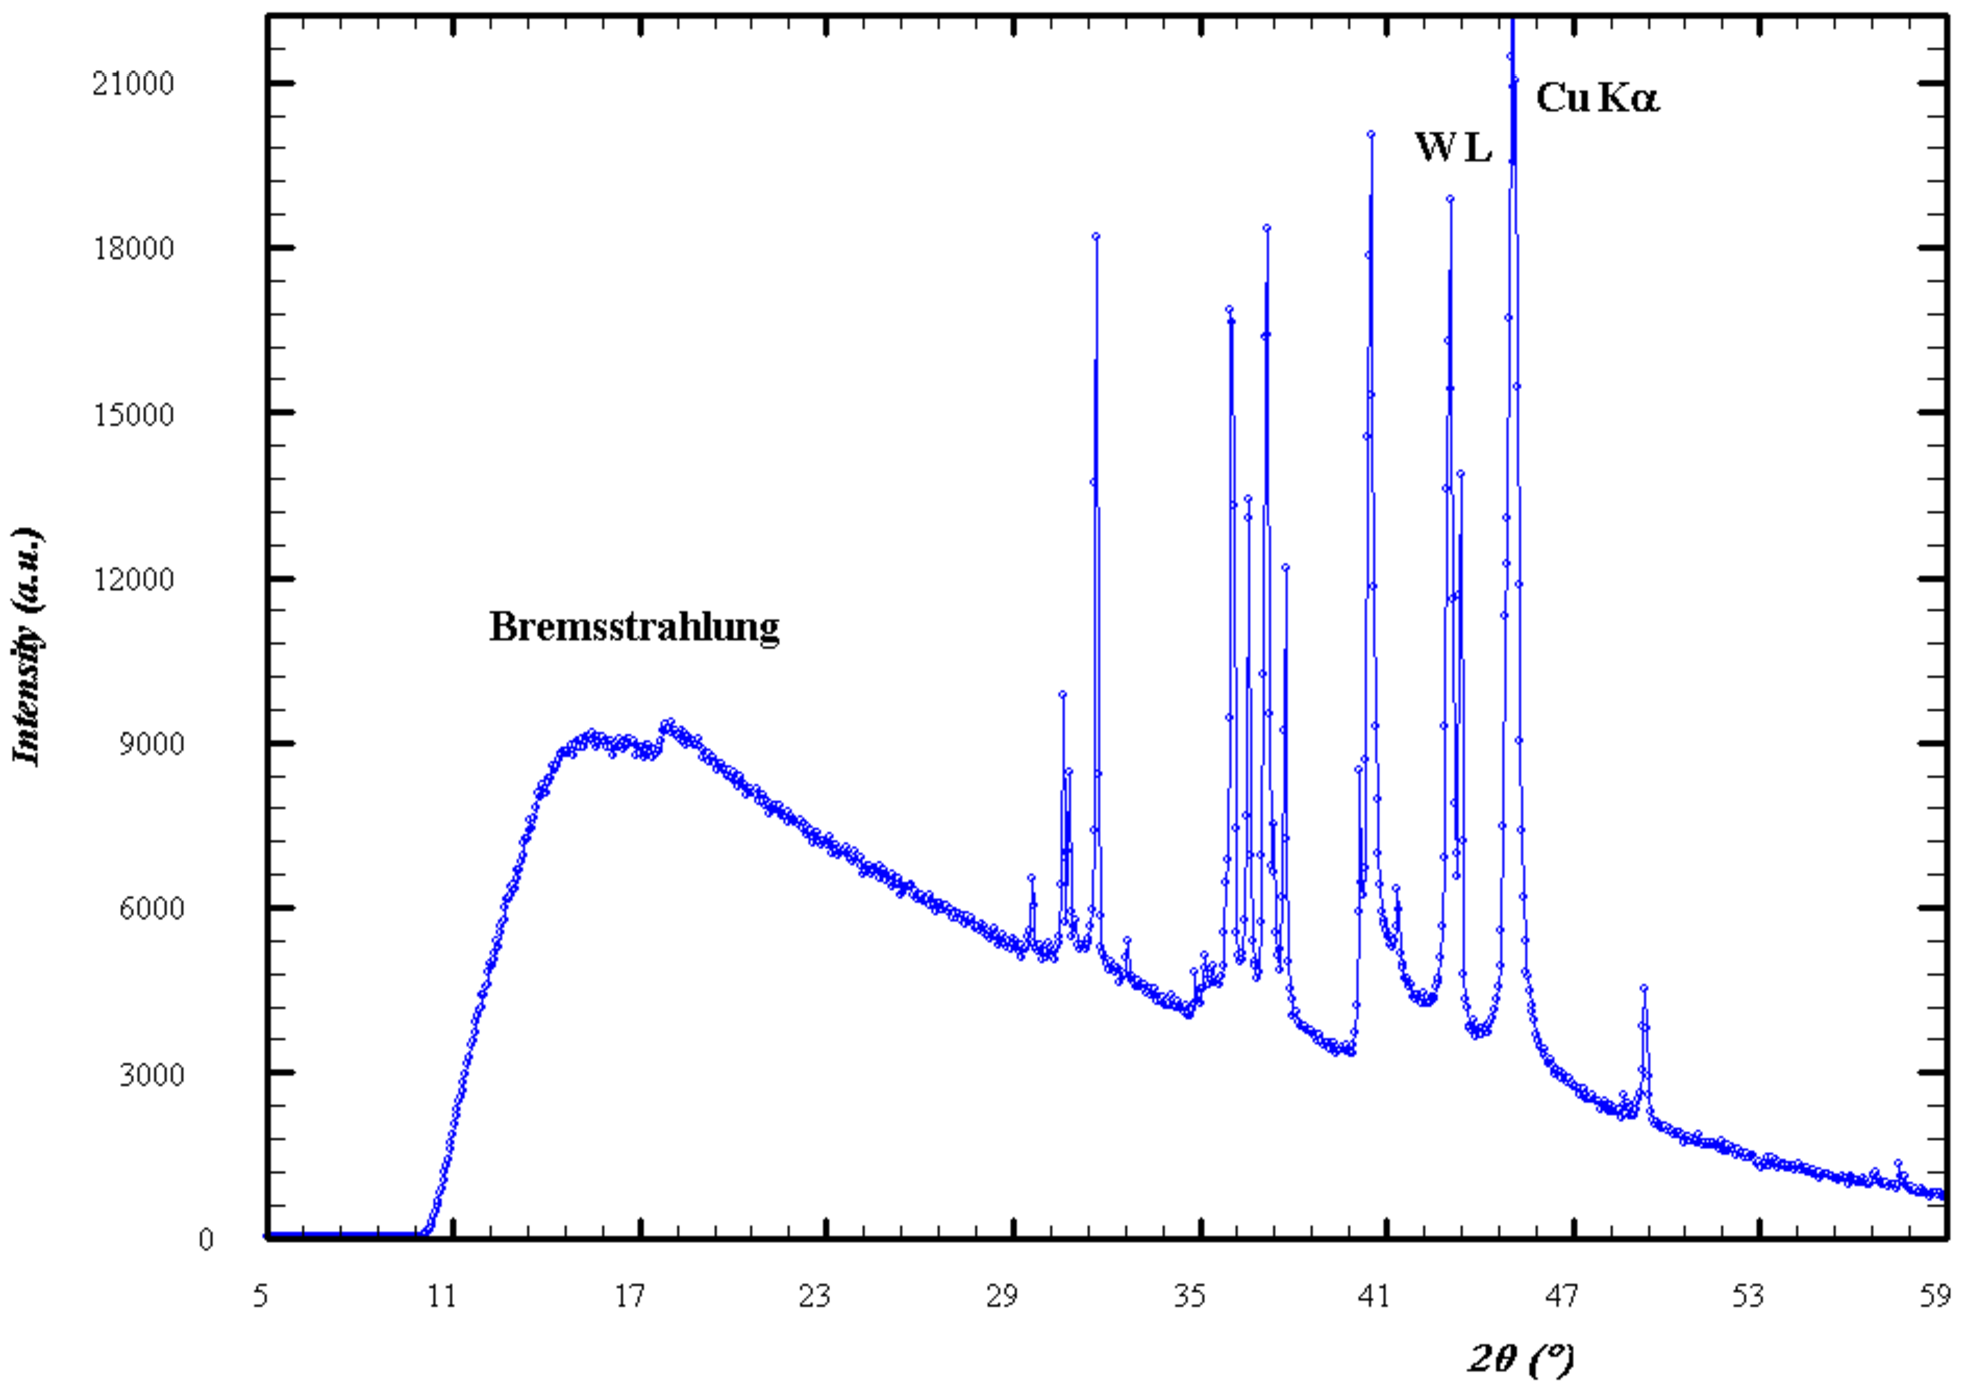
\includegraphics[width=1\textwidth]{./figures/Tube_Cu_LiF.pdf}
	\caption{Charakteristisches Spektrum einer Kupferanode nach Bragg-Reflexion an einem LiF-Kristall. Der Untergrund entsteht aufgrund der emittierten Bremsstrahlung der in der Anode gestreuten Elektronen. Auf diesem liegt das charakteristische Röntgenspektrum der Anode. Quelle: \url{http://commons.wikimedia.org/wiki/File:Tube_Cu_LiF.PNG} (Letzter Zugriff: 13. November 2014)}
	\label{fig:spektrum}
\end{figure}

Eine \textbf{Röntgenröhre} (schematisch in Abbildung \ref{fig:roehre}) besteht aus einem evakuierten Glaskolben mit einer Anordnung von geheizter Kathode und Anode aus Targetmaterial.
Zwischen Kathode und Anode wird die Beschleunigungsspannung $U$ angelegt, sodass beim Heizen der Kathode mit der Heizspannung $U_\mathrm{Heiz}$ aufgrund des glühelektrischen Effekts ein Teil der Elektronen die Austrittsarbeit der Kathode überwinden kann und durch die Beschleunigungsspannung $U$ in Richtung der Anode beschleunigt werden.
Nachdem die Beschleunigungsspannung $U$ durchlaufen wurde, treffen die Elektronen mit der Energie $e U$ auf das Anodenmaterial und erzeugen dabei Bremsstrahlung sowie charakteristische Strahlung, welche durch ein für Röntgenstrahlung durchlässiges Fenster im Glaskolben aus der Röhre austreten können.
\begin{figure}[ht]
	\centering
	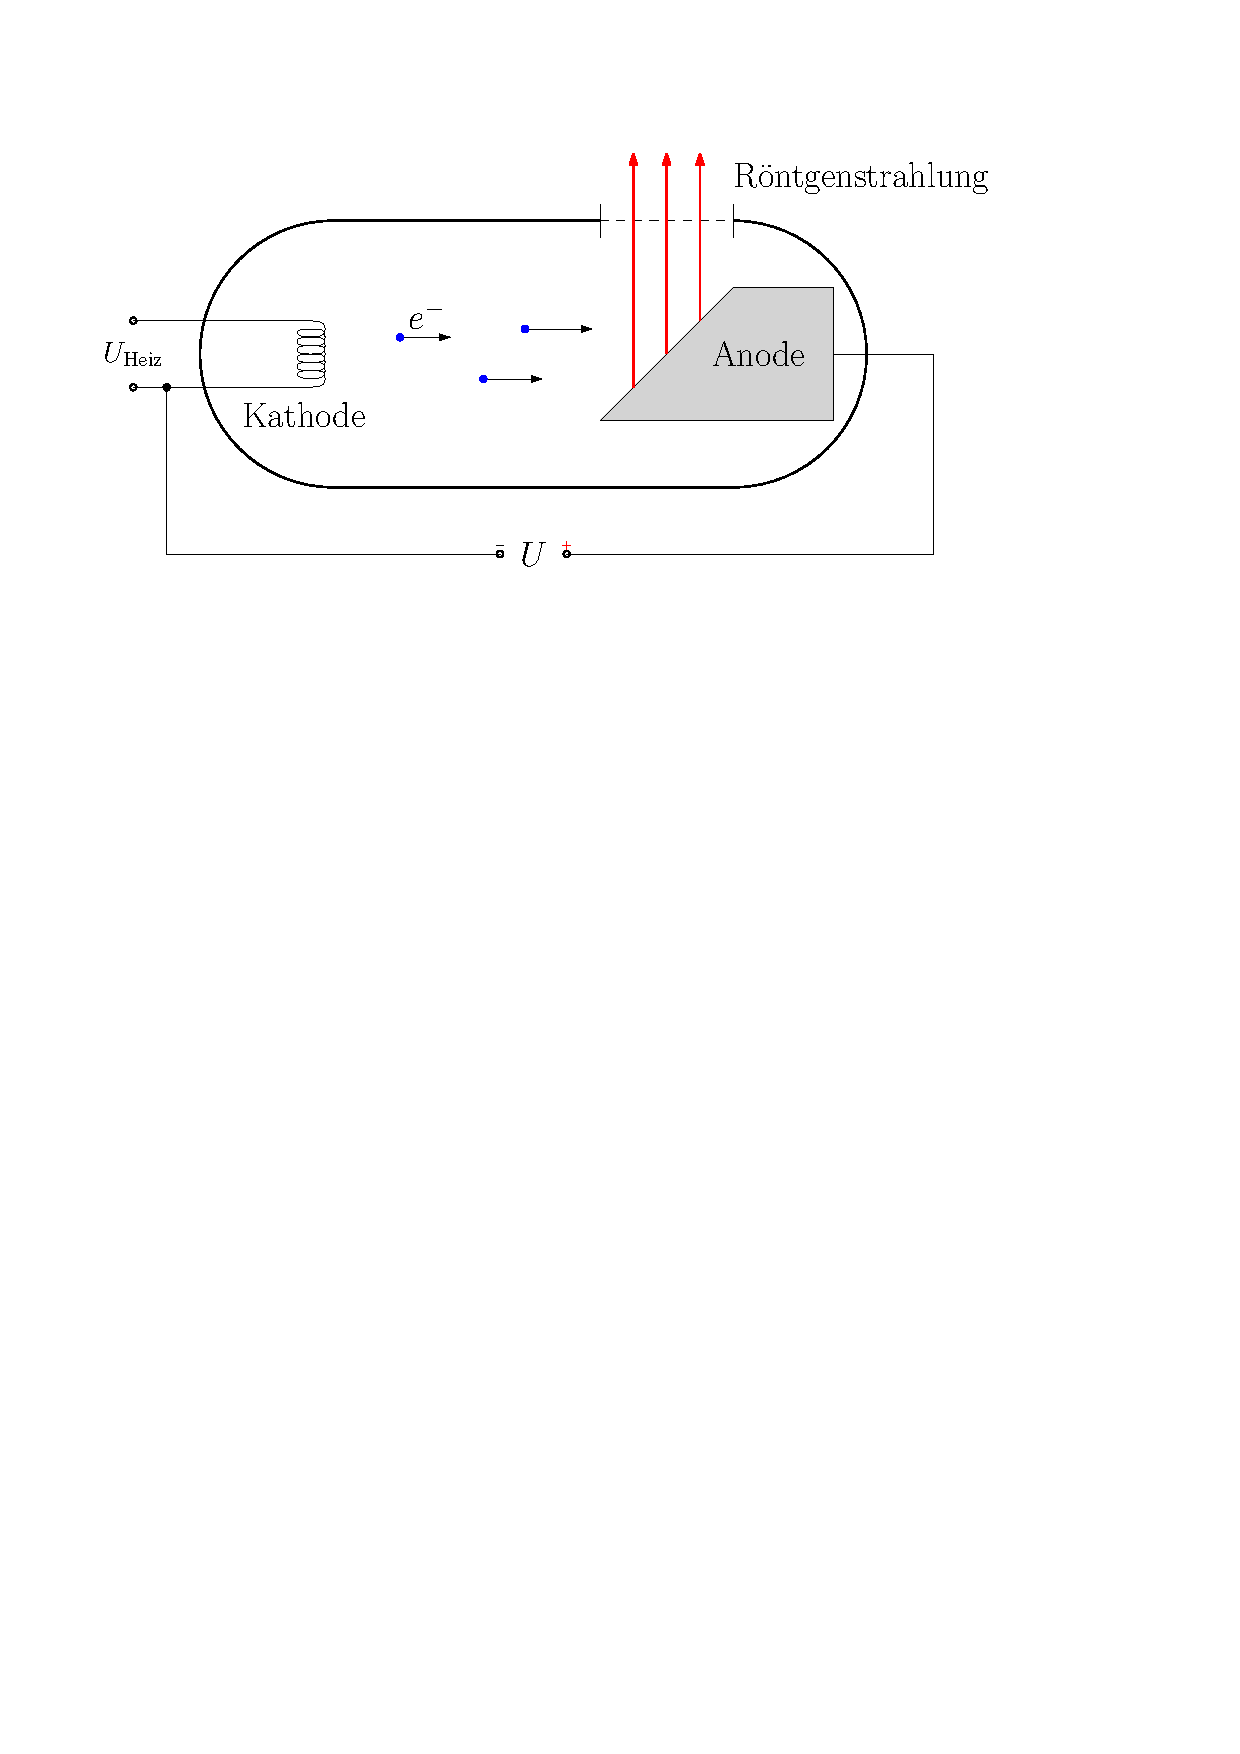
\includegraphics[width=0.75\textwidth]{./figures/roentgenroehre.pdf}
	\caption{schematischer Aufbau einer Röntgenröhre}
	\label{fig:roehre}
\end{figure}

\subsection{Röntgenstrahlung}

\subsubsection{Erzeugung und Nachweis}
NACHWEIS:
\begin{itemize}
	\item \textbf{Lumineszenz:} Bestimmte Stoffe werden durch Röntgenstrahlung zur Emission von Licht angeregt.
	
	\item \textbf{Photographischer Effekt:} Röntgenstrahlung schwärzt einen Röntgenfilm direkt.
	
	\item \textbf{Szintillationszähler, Halbleiterdetektoren, Geigerzähler}
\end{itemize}

\subsubsection{kontinuierliches und charakteristisches Röntgenspektrum}


\subsection{Geiger-Müller-Zählrohr}
Das Geiger-Müller-Zählrohr besteht aus einem Metallzylinder, der die Kathode darstellt und einem Draht im Inneren des Zylinders, der die Anode bildet.
Der Zylinder ist mit einem Gas unter hohem Druck gefüllt, wobei meistens ein Edelgas verwendet wird, da dieses keine negativen Ionen bildet, die den Betrieb stören können.
Bei Eintritt von Teilchen in das Zählrohr werden die Gasatome im Inneren ionisiert und so freie Elektronen und positiv geladene Ionen erzeugt.
Durch die zwischen Draht und Zylindermantel anliegende Spannung werden die Elektronen zum Draht beschleunigt, die Ionen aufgrund ihrer höheren Masse deutlich langsamer zum Mantel hin.

Für den Betrieb ist die angelegte Gleichspannung zwischen Anode und Kathode entscheidend:
Bei geringer Spannung können die freien Elektronen auf der Beschleunigungsstrecke wieder mit den Ionen rekombinieren, wodurch der gemessene Stromimpuls nur von den Elektronen erzeugt wird, die die Anode erreichen.
So kann keine verlässliche Aussage über die einfallende Strahlung gemacht werden (\emph{Rekombinationsbereich}).
Erst ab einer bestimmten Gleichspannung ($\sim \SI{100}{\volt}$) erreichen alle Elektronen die Anode, womit dann die von der Strahlung im Zählrohr abgegebene Energie gemessen wird (\emph{Ionisationskammer}).
Erhöht man die Spannung weiter erreicht man den \emph{Proportionalitätsbereich}.
Hier werden die Elektronen so stark beschleunigt, dass sie auf dem Weg zum Draht genug Energie gewinnen, um weitere Gasatome zu ionisieren.
So entsteht ein Lawineneffekt, der den gemessenen Stromimpuls deutlich vergrößert (bei $n$ Elektronen pro Lawine ist dieser $n$-mal größer) und so genauere Messungen als in der Ionisationskammer ermöglicht.
Beim \emph{Geiger-Müller-Bereich} ist die angelegte Spannung so hoch, dass die Elektronen, ähnlich wie im Proportionalitätsbereich, weitere Atome ionisieren können, und dass die dabei entstandenen Elektronen wieder Atome ionisieren.
Der Lawineneffekt wird also deutlich verstärkt und eine selbstständige Gasentladung ausgelöst.
Diese endet erst, wenn sich durch die entstandenen, positiv geladenen Ionen, die (langsam) zum Mantel des Zylinders beschleunigt werden, eine Raumladungszone im Rohr ausbildet, die die Feldstärke verringert.
Zur Auslösung wird nur ein einzelnes Ereignis benötigt, wodurch das Geiger-Müller-Zählrohr maximale Empfindlichkeit besitzt.
Die gemessenen Stromimpulse sind durch die hohe Beschleunigungsspannung, die die Elektronen erfahren, alle gleich groß, es wird also nur die Anzahl und nicht die Energie der einfallenden Strahlung gemessen.
Durch den angesprochenen Effekt der selbstständigen Gasentladung hat das Geiger-Müller-Zählrohr eine s.g. \emph{Totzeit}, welche beschreibt, wie lange keine neu einfallende Strahlung gemessen werden kann, da die Gasatome vorher beinahe alle ionisiert sind und erst wieder mit den Elektronen rekombinieren müssen.

\subsubsection{Aufbau}

\subsubsection{Funktionsweise}

\subsubsection{Totzeit und Totzeitkorrektur}
Endliche Zeit des Detektors ein Signal zu verarbeiten lässt ihn insensitiv für neue Ereignisse.
Man unterscheidet zwischen Paralysierenden und Nicht-Paralysierenden Systemen.
Bei nicht-paralysierendem Verhalten führt ein zweites Ereignis lediglich zum Verlust dieses Ereignisses.
Bei paralysierendem Verhalten führt ein zweites Event zum "Neustart" der Totzeit.
Bei semi-paralysierendem Verhalten erhöht ein zweites Event lediglich die Zeit in der der Detektor nicht sensitiv ist (aber nicht um die Länge der Totzeit).

(Cite Leo)Unter Annahme eines nicht paralysierenden Systems (Totzeit: $\tau$) mit der wahren Count-Rate $m$ und der vom Detektor gezählten Anzahl der Events $k$ in einer Zeit $T$.
Da jeder Count eine Totzeit auslöst ergibt sich die gesamte Totzeit zu:
\begin{align}
	\tau_\mathrm{ges.} = k \cdot \tau
\end{align}
In dieser Zeit verpasst man $m k \tau$ Events.
Dadurch ergibt sich:
\begin{align}
	m T = k + m k \tau
\end{align}
und auflösen nach $m$:
\begin{align}
	m = \frac{k / T}{1 - (k/T) \tau}
\end{align}

Unter Annahme eines paralysierenden Systems werden nur Events gezählt zwischen denen eine Zeit von $\tau$ liegt.
Die Verteilung der Zeitintervalle zwischen zwei Zerfällen ist:
\begin{align}
	P(t) = m \, \mathrm{e}^{-m t}
\end{align}
mit der Wahrscheinlichkeit für $t > \tau$:
\begin{align}
	P(t>\tau) = m \int_{\tau}^{\infty} \mathrm{e}^{-m t} \, \mathrm{d}t = \mathrm{e}^{-m \tau}
\end{align}
Dann ist die tatsächlich gemessene Rate $k$:
\begin{align}
	k = m T \, \mathrm{e}^{-m \tau}
\end{align}
Diese Gleichung hat zwei Lösungen!
Die kleinere der Lösungen liegt auf der mit $m$ ansteigenden Zählrate $k/T$ und die größere der Lösungen liegt auf der abfallenden Flanke.
SIEHE BILD LEO S.124 Fig.5.5!!!
Plotten von Zählrate für paralysierende Systeme und nichtparalysierende Systeme (Christopher weiß bescheid)!


\subsection{Dosimetrische Messgrößen}

\subsubsection{Aktivität}
Zerfallsgesetz:
\begin{align}
	\frac{\mathrm{d} N(t)}{\mathrm{d} t} = - \lambda \cdot N(t)
\end{align}
beschreibt die Abnahme von Teilchen.
Aktivität beschreibt die Anzahl der Zerfälle pro Zeiteinheit also:
\begin{align}
	A(t) = - \frac{\mathrm{d} N(t)}{\mathrm{d} t} = \lambda \cdot N(t)
\end{align}

\subsubsection{Energiedosis}
Die im Absorberelement $\mathrm{d}V$ mit der Masse $\mathrm{d} m = \rho \cdot \mathrm{d}V$ deponierte Energie $\mathrm{d}E$:
\begin{align}
	D &= \frac{\mathrm{d}E}{\mathrm{d}m} = \frac{1}{\rho}\frac{\mathrm{d}E}{\mathrm{d}V}\\
	[D] &= \frac{\mathrm{J}}{\mathrm{kg}} = \mathrm{Gy} \quad \text{(Gray)}
\end{align}
Physikalische nicht biologische Größe.

\subsubsection{Ionendosis}
Bezeichnet die elektrische Ladung die durch ionisierende Strahlung in einer bestimmten Masse entsteht:
\begin{align}
	J = \frac{\mathrm{d}Q}{\mathrm{d}m}
\end{align}
Kann durch Kenntnis der mittleren Energie für die Bildung eines Ionenpaares in Energiedosis umgerechnet werden.

\subsubsection{Dosisleistung}
\begin{align}
	\dot{D} = \frac{\mathrm{d}D}{\mathrm{d}t}
\end{align}

\subsubsection{Äquivalentdosis}
Äquivalentdosis $H$.
Beachtet die relative biologische Wirksamkeit verschiedener Strahlungstypen durch Einführung eines Qualitätsfaktors $Q$.
\begin{align}
	H = Q \cdot D
\end{align}
Die Äquivalentdosis hat die gleiche Einheit wie die Dosis und wird daher um die physikalische Größe der Dosis von der Biologischen der Äquivalentdosis zu unterscheiden mit Sievert "beeinheitet".

Typische Qualitätsfaktoren (Gerthsen):
\begin{align*}
	&\text{Strahlungsart} \quad & Q / \si{Sv.Gy\tothe{-1}}\\
	&\text{Röntgen- und Gammastrahlung} \quad & 1 \\
	&\text{Betastrahlung} \quad & 1 \\
	&\text{Schnelle Neutronen} \quad & 10 \\
	&\text{Langsame Neutronen} \quad & 5 \\
	&\text{Alphastrahlung} \quad & 10 \\
	&\text{Schwere Rückstoßkerne} \quad & 20
\end{align*}


\subsection{Bildkontrast, Bildhelligkeit und visuelle Ortsauflösung}


\subsection{4-A Regel im Strahlenschutz}
\begin{itemize}
	\item \textbf{Abstand:}
	Die Wirkung von ionisierender Strahlung sinkt stark mit dem Abstand von der Quelle ($1/r^2$-Gesetz) und sollte daher stehts maximiert werden.
	Z.B. durch Sperrbereiche, ausgestrecktem Arm und andere Haltewerkzeuge (Zangen).
	
	
	\item \textbf{Aufenthaltszeit:}
	Die zugeführte Dosis ist proportional zur Aufenthaltszeit und sollte damit minimiert werden.
	
	
	\item \textbf{Abschirmung:}
	Durch geeignete Abschirmung kommt es zu einem exponentiellen Abfall der Strahlungsintensität im Absorber (Lambert-Beer-Gesetz).
		
	
	\item \textbf{Aktivität:}
	Die Aktivität eines Präparats sollte bekannt sein und wenn möglich minimiert werden.
	D.h. wenn es das Experiment erlaubt sollte ein Präparat geringerer Aktivität verwendet werden.
	
	
\end{itemize}


\subsection{Aufbau und Funktionsweise verschiedener Personendosimeter}

\subsubsection{Füllhalterdosimeter (Quartz fiber dosimeter)}
(Veraltet)
\begin{itemize}
	\item Geringe Genauigkeit: analog/mechanisches Design
	\item Ablesefehler
	\item Kleiner Messbereich (große Dosen sättigen)
	\item Feuchtigkeitsempfindlich
\end{itemize}
Besteht aus einer zylinderförmigen mit Luft gefüllten Ionisationskammer in der sich ein Elektrodendraht befindet.
Am Ende der Elektrode ist eine Quartzfaser welche parallel zur Elektrode ruht und leitend mit der Elektrode verbunden ist.
Lädt man die Elektrode auf, so stößt sich die Quartzfaser von der Elektrode ab.
Die Position der Quartzfaser kann mit einem angebrachten Mikroskop abgelesen werden.
Tritt eine Ionisation in der Kammer auf, so wird ein Teil der Ladung auf der Elektrode neutralisiert und die Quartzfaser nähert sich der Elektrode aufgrund der verringerten Abstoßung.
Dies ist ein Maß für die erhaltene Dosis.

\subsubsection{Filmdosimeter}
Besteht aus Halter und photographischem Film.\\
Zum Messen der Dosis wird der Film entwickelt. Bestrahlung erhöht die optische Dichte des entwickelten Films (es schwärzt sich).\\
Oft mehrere Filme mit verschiedenen dynamischen Bereichen um den Messbereich der Dosis zu maximieren.\\
Sensitiv auf Gamma, Röntgen und Beta-Strahlung.\\
Der Halter enthält verschiedene Filter für gewisse Strahlungstypen um zwischen den Typen unterscheiden zu können und die Äquivalentdosis berechnen zu können.\\
\begin{itemize}
	\item Gamma: Aluminium oder Kupferfilter
	\item Beta: Plastik verschiedener Dichte
\end{itemize}

\subsubsection{Thermolumineszenzdosimeter (TLD)}
Ausnutzung von Thermolumineszenz: bestimmte kristalline Stoffe emittieren beim erhitzen Licht (keine Schwarzkörperstrahlung!) abhängig von der vorigen Bestrahlung mit elektromagnetischer oder ionisierender Strahlung.
Die Intensität dieser Strahlung ist abhängig von der Strahlenbelastung.

\subsubsection{Electronic Personal Dosimeter}
Elektronische Geräte die mithilfe von Halbleiterdetektoren (PIN-Diode, MOSFETs) die Energie von einfallender Strahlung bestimmen.\\
\\
\textbf{PIN-Diode:} Dotiertes Halbleiterstück in P-I(Intrinsisch)-N\\
In der Verarmungszone kann durch einfallende ionisierende Strahlung eine Elektron-Loch Kaskade entstehen wobei die ausgelöste Ladung proportional zur Energie des absorbierten Quants ist.\\
Mithilfe eines Integrators kann damit die Energie bestimmt werden und die Dosis berechnet werden.\\
\\
\textbf{MOSFET:} Die Grenzspannung zum Durchschalten des MOSFET $V_\mathrm{TH}$.\\
Wird der MOSFET bestrahlt so bildet sich gefangene Ladung im Oxid des MOSFET und es werden Elektronen-Loch Paare erzeugt.
Durch die geringere Mobilität der Löcher werden diese im Halbleitermaterial gefangen und führen zu einer negativen Spannungsverschiebung der Grenzspannung $\Delta V_\mathrm{TH}$.
Die Spannungsverschiebung ist proportional zur Dosis.


\subsection{Abschwächung von Röntgenstrahlen (Lambertsches Schwächungsgesetz)}
Beschreibt Abschwächung der Intensität von Strahlung in einem Absorber durch Streuung und Absorption.
Trifft auf einen infinitesimalen Absorber der Dicke $\mathrm{d} x$ Strahlung der Intensität $I$, so kommt es zur Änderung der Strahlungsintensität hinter dem Absorber um:
\begin{align}
	\mathrm{d} I = - \alpha I \mathrm{d} x
\end{align}
Dabei beschreibt $\alpha$ den materialabhängigen Absorptionskoeffizienten, welcher von der Strahlungenergie abhängt.
Gemäß der Differentialgleichung ist das Lambertsche Schwächungsgesetz gegeben durch:
\begin{align}
	I(x) = I_0 \, \mathrm{e}^{-\alpha x}
\end{align}

Oftmals alternative Darstellung durch die Transmission $T = I(x)/I_0$:
\begin{align}
	T = \mathrm{e}^{-\mu x}
\end{align}
wobei $\mu = \alpha$ der lineare Schwächungskoeffizient ist.

(WIKI:) Für Energien über \SI{50}{keV} gilt:
je weniger dicht und je weniger klein $Z$ desto geringer ist $\mu$. Daher ist Blei beliebtes Material zur Abschirmung.

\section{Versuchsaufbau}

\section{Durchführung und Auswertung}
Die ausführliche Durchführung ist der Versuchsanleitung \cite{anleitung} zu entnehmen.
Sollten Abweichungen bei der Durchführung auftreten, so werden diese im jeweiligen Unterkapitel dargestellt.

\subsection{Dosimetrie}

\subsubsection{Plattenkondensator als Ionisationskammer}
In diesem Versuchsteil soll die Verwendung eines Plattenkondensators als Ionisationskammer überprüft werden.
Dazu wird der Plattenkondensator im Experimentierraum des Röntgengeräts installiert, sodass sich dessen Zwischenraum im Strahlungsfeld der Molybdän-Röntgenröhre befindet.
Um eine Ionisationskammer zu realisieren, wird an den Kondensator eine variable Gleichspannung $U_\mathrm{C}$ angelegt, welche die durch die Röntgenstrahlung erzeugten Ionen zu den Kondensatorplatten driften lässt.
Sollte die im Kondensator erzeugte Ladung eine der Platten erreichen, so kann dies als Ionisationsstrom $I_\mathrm{C}$ in der äußeren Beschaltung gemessen werden.
Der Ionisationsstrom kann dann als Spannung $U_{I_\mathrm{C}}$ an einem Messwiderstand $R$ gemessen werden:
\begin{align}
	I_\mathrm{C} = \frac{U_{I_\mathrm{C}}}{R}
	\label{eq:ohm_ionisationsstrom}
\end{align}
Da die auftretenden Ströme in der Größenordnung einiger \si{nA} liegen, muss ein dementsprechend hochohmiger Widerstand verwendet werden, was zur Folge hat, dass die Spannung nicht mit einem einfachen Voltmeter gemessen werden kann, da diese einen geringeren Innenwiderstand haben als der verwendete Messwiderstand.
Daher wird ein Elektrometerverstärker mit einfacher Verstärkung verwendet, um die Spannung belastungsfrei am Messwiderstand mit einem Multimeter messen zu können.

Folglich soll der Ionisationsstrom $I_\mathrm{C}$ in Abhängigkeit der Kondensatorspannung $U_\mathrm{C}$ für verschiedene Röhrenspannungen $U$ bestimmt werden.
Dabei wird der Emissionsstrom\footnote{Der Fehler des Emissionsstroms wird anhand der letzten Stelle der Digitalanzeige des Röntgengeräts auf \SI{0.01}{\milli\ampere} abgeschätzt.} $I$ der Röntgenröhre auf \SI{1.00 +- 0.01}{mA} eingestellt und ein Messwiderstand $R = \SI{1}{\giga\ohm}$ verwendet, wobei auf den Widerstand ein relativer Fehler von \SI{1}{\percent} angenommen wird.
Dann ergibt sich der Ionisationsstrom durch Gleichung \ref{eq:ohm_ionisationsstrom} und der Fehler durch Gauß'sche Fehlerfortpflanzung:
\begin{align}
	\Delta I_\mathrm{C} = \sqrt{\frac{\Delta U_{I_\mathrm{C}}^2}{R^2} + \frac{U_{I_\mathrm{C}}^2 \cdot \Delta R^2}{R^4}}
\end{align}
wobei der Fehler der Spannungsmessung am Elektrometerverstärker anhand des Rauschen am Verstärkers für jede Messung einzeln abgeschätzt wird.
Darüber hinaus wird die variable Gleichspannung $U_\mathrm{C}$ direkt mit einem weiteren Multimeter gemessen und der Fehler im Messbereich \num{0} bis \SI{400}{V} auf \SI{0.1}{V} abgeschätzt.


\begin{figure}[ht]
	\centering
	% GNUPLOT: LaTeX picture with Postscript
\begingroup
  \makeatletter
  \providecommand\color[2][]{%
    \GenericError{(gnuplot) \space\space\space\@spaces}{%
      Package color not loaded in conjunction with
      terminal option `colourtext'%
    }{See the gnuplot documentation for explanation.%
    }{Either use 'blacktext' in gnuplot or load the package
      color.sty in LaTeX.}%
    \renewcommand\color[2][]{}%
  }%
  \providecommand\includegraphics[2][]{%
    \GenericError{(gnuplot) \space\space\space\@spaces}{%
      Package graphicx or graphics not loaded%
    }{See the gnuplot documentation for explanation.%
    }{The gnuplot epslatex terminal needs graphicx.sty or graphics.sty.}%
    \renewcommand\includegraphics[2][]{}%
  }%
  \providecommand\rotatebox[2]{#2}%
  \@ifundefined{ifGPcolor}{%
    \newif\ifGPcolor
    \GPcolortrue
  }{}%
  \@ifundefined{ifGPblacktext}{%
    \newif\ifGPblacktext
    \GPblacktexttrue
  }{}%
  % define a \g@addto@macro without @ in the name:
  \let\gplgaddtomacro\g@addto@macro
  % define empty templates for all commands taking text:
  \gdef\gplbacktext{}%
  \gdef\gplfronttext{}%
  \makeatother
  \ifGPblacktext
    % no textcolor at all
    \def\colorrgb#1{}%
    \def\colorgray#1{}%
  \else
    % gray or color?
    \ifGPcolor
      \def\colorrgb#1{\color[rgb]{#1}}%
      \def\colorgray#1{\color[gray]{#1}}%
      \expandafter\def\csname LTw\endcsname{\color{white}}%
      \expandafter\def\csname LTb\endcsname{\color{black}}%
      \expandafter\def\csname LTa\endcsname{\color{black}}%
      \expandafter\def\csname LT0\endcsname{\color[rgb]{1,0,0}}%
      \expandafter\def\csname LT1\endcsname{\color[rgb]{0,1,0}}%
      \expandafter\def\csname LT2\endcsname{\color[rgb]{0,0,1}}%
      \expandafter\def\csname LT3\endcsname{\color[rgb]{1,0,1}}%
      \expandafter\def\csname LT4\endcsname{\color[rgb]{0,1,1}}%
      \expandafter\def\csname LT5\endcsname{\color[rgb]{1,1,0}}%
      \expandafter\def\csname LT6\endcsname{\color[rgb]{0,0,0}}%
      \expandafter\def\csname LT7\endcsname{\color[rgb]{1,0.3,0}}%
      \expandafter\def\csname LT8\endcsname{\color[rgb]{0.5,0.5,0.5}}%
    \else
      % gray
      \def\colorrgb#1{\color{black}}%
      \def\colorgray#1{\color[gray]{#1}}%
      \expandafter\def\csname LTw\endcsname{\color{white}}%
      \expandafter\def\csname LTb\endcsname{\color{black}}%
      \expandafter\def\csname LTa\endcsname{\color{black}}%
      \expandafter\def\csname LT0\endcsname{\color{black}}%
      \expandafter\def\csname LT1\endcsname{\color{black}}%
      \expandafter\def\csname LT2\endcsname{\color{black}}%
      \expandafter\def\csname LT3\endcsname{\color{black}}%
      \expandafter\def\csname LT4\endcsname{\color{black}}%
      \expandafter\def\csname LT5\endcsname{\color{black}}%
      \expandafter\def\csname LT6\endcsname{\color{black}}%
      \expandafter\def\csname LT7\endcsname{\color{black}}%
      \expandafter\def\csname LT8\endcsname{\color{black}}%
    \fi
  \fi
    \setlength{\unitlength}{0.0500bp}%
    \ifx\gptboxheight\undefined%
      \newlength{\gptboxheight}%
      \newlength{\gptboxwidth}%
      \newsavebox{\gptboxtext}%
    \fi%
    \setlength{\fboxrule}{0.5pt}%
    \setlength{\fboxsep}{1pt}%
\begin{picture}(7200.00,5040.00)%
    \gplgaddtomacro\gplbacktext{%
      \csname LTb\endcsname%
      \put(550,704){\makebox(0,0)[r]{\strut{}$0$}}%
      \csname LTb\endcsname%
      \put(550,1383){\makebox(0,0)[r]{\strut{}$1$}}%
      \csname LTb\endcsname%
      \put(550,2061){\makebox(0,0)[r]{\strut{}$2$}}%
      \csname LTb\endcsname%
      \put(550,2740){\makebox(0,0)[r]{\strut{}$3$}}%
      \csname LTb\endcsname%
      \put(550,3418){\makebox(0,0)[r]{\strut{}$4$}}%
      \csname LTb\endcsname%
      \put(550,4097){\makebox(0,0)[r]{\strut{}$5$}}%
      \csname LTb\endcsname%
      \put(550,4775){\makebox(0,0)[r]{\strut{}$6$}}%
      \csname LTb\endcsname%
      \put(682,484){\makebox(0,0){\strut{}$0$}}%
      \csname LTb\endcsname%
      \put(1447,484){\makebox(0,0){\strut{}$50$}}%
      \csname LTb\endcsname%
      \put(2212,484){\makebox(0,0){\strut{}$100$}}%
      \csname LTb\endcsname%
      \put(2977,484){\makebox(0,0){\strut{}$150$}}%
      \csname LTb\endcsname%
      \put(3743,484){\makebox(0,0){\strut{}$200$}}%
      \csname LTb\endcsname%
      \put(4508,484){\makebox(0,0){\strut{}$250$}}%
      \csname LTb\endcsname%
      \put(5273,484){\makebox(0,0){\strut{}$300$}}%
      \csname LTb\endcsname%
      \put(6038,484){\makebox(0,0){\strut{}$350$}}%
      \csname LTb\endcsname%
      \put(6803,484){\makebox(0,0){\strut{}$400$}}%
    }%
    \gplgaddtomacro\gplfronttext{%
      \csname LTb\endcsname%
      \put(176,2739){\rotatebox{-270}{\makebox(0,0){\strut{}Ionisationsstrom $I_\mathrm{C} / \si{nA}$}}}%
      \put(3742,154){\makebox(0,0){\strut{}Kondensatorspannung $U_\mathrm{C} / \si{V}$}}%
      \csname LTb\endcsname%
      \put(2266,4602){\makebox(0,0)[r]{\strut{}$U_\mathrm{C} = \SI{15}{kV}$}}%
      \csname LTb\endcsname%
      \put(2266,4382){\makebox(0,0)[r]{\strut{}$U_\mathrm{C} = \SI{25}{kV}$}}%
      \csname LTb\endcsname%
      \put(2266,4162){\makebox(0,0)[r]{\strut{}$U_\mathrm{C} = \SI{35}{kV}$}}%
    }%
    \gplbacktext
    \put(0,0){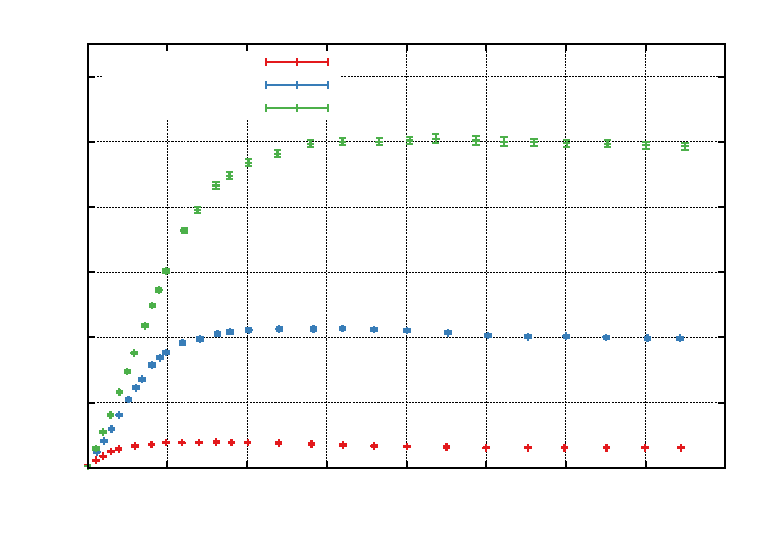
\includegraphics{./plots/kondensatorspannung}}%
    \gplfronttext
  \end{picture}%
\endgroup

	\label{fig:kondensatorspannung}
	\caption{Abhängigkeit des Ionisationsstroms $I_\mathrm{C}$ von der Kondensatorspannung $U_\mathrm{C}$}
\end{figure}

\subsubsection{Abhängigkeit des Ionisationsstromes vom Emissionsstrom der Röntgenröhre}

\subsubsection{Bestimmung der Ionendosisleistung im Kondensator}

\subsubsection{Bestimmung der Dosisleistung mit einem Stabdosimeter}

\subsubsection{Überprüfung des Abstandsquadratgesetzes}


\subsection{Totzeit}

Da bei den weiteren Messungen das Geiger-Müller-Zählrohr verwendet wird, ist es notwendig, zunächst seine Totzeit abzuschätzen.
Dazu wird das Zählrohr auf dem Goniometer befestigt und zur Bestrahlung eine Röntgenröhre aus Kupfer mit davor sitzendem Kollimator (bei diesem Versuch wurde der Kollimator mit breitem Spalt verwendet) genutzt.
Das Zählrohr wird so positioniert, dass es sich gleich weit von der Goniometermitte entfernt befindet wie der Kollimator von der Goniometermitte (je ca. \num{5} bis \SI{7}{cm}).
Zur Messung wird die Zählrate über $\Delta t=\SI{30}{\second}$ gemittelt und eine Röhrenspannung von $U=\SI{35}{\kilo\volt}$ fest eingestellt, während der Emissionsstrom $I_\text{E}$ von \num{0} bis \SI{1}{\milli\ampere} variiert wird.
Das Maximum der Zählrate wird bei einer Winkeleinstellung des Zählrohrs von $\beta=\SI{-0.9}{\degree}$ lokalisiert und das Zählrohr für alle folgenden Messungen auf dieser Einstellung genutzt.
Die so gefundenen Zählraten in Abhängigkeit des Emissionsstroms sind in Tabelle REF festgehalten.
TABELLE
Grafisch aufgetragen erhält man aus diesen die Abbildung \ref{fig:totzeit}
\begin{figure}[ht]
	\centering
	% GNUPLOT: LaTeX picture with Postscript
\begingroup
  \makeatletter
  \providecommand\color[2][]{%
    \GenericError{(gnuplot) \space\space\space\@spaces}{%
      Package color not loaded in conjunction with
      terminal option `colourtext'%
    }{See the gnuplot documentation for explanation.%
    }{Either use 'blacktext' in gnuplot or load the package
      color.sty in LaTeX.}%
    \renewcommand\color[2][]{}%
  }%
  \providecommand\includegraphics[2][]{%
    \GenericError{(gnuplot) \space\space\space\@spaces}{%
      Package graphicx or graphics not loaded%
    }{See the gnuplot documentation for explanation.%
    }{The gnuplot epslatex terminal needs graphicx.sty or graphics.sty.}%
    \renewcommand\includegraphics[2][]{}%
  }%
  \providecommand\rotatebox[2]{#2}%
  \@ifundefined{ifGPcolor}{%
    \newif\ifGPcolor
    \GPcolortrue
  }{}%
  \@ifundefined{ifGPblacktext}{%
    \newif\ifGPblacktext
    \GPblacktexttrue
  }{}%
  % define a \g@addto@macro without @ in the name:
  \let\gplgaddtomacro\g@addto@macro
  % define empty templates for all commands taking text:
  \gdef\gplbacktext{}%
  \gdef\gplfronttext{}%
  \makeatother
  \ifGPblacktext
    % no textcolor at all
    \def\colorrgb#1{}%
    \def\colorgray#1{}%
  \else
    % gray or color?
    \ifGPcolor
      \def\colorrgb#1{\color[rgb]{#1}}%
      \def\colorgray#1{\color[gray]{#1}}%
      \expandafter\def\csname LTw\endcsname{\color{white}}%
      \expandafter\def\csname LTb\endcsname{\color{black}}%
      \expandafter\def\csname LTa\endcsname{\color{black}}%
      \expandafter\def\csname LT0\endcsname{\color[rgb]{1,0,0}}%
      \expandafter\def\csname LT1\endcsname{\color[rgb]{0,1,0}}%
      \expandafter\def\csname LT2\endcsname{\color[rgb]{0,0,1}}%
      \expandafter\def\csname LT3\endcsname{\color[rgb]{1,0,1}}%
      \expandafter\def\csname LT4\endcsname{\color[rgb]{0,1,1}}%
      \expandafter\def\csname LT5\endcsname{\color[rgb]{1,1,0}}%
      \expandafter\def\csname LT6\endcsname{\color[rgb]{0,0,0}}%
      \expandafter\def\csname LT7\endcsname{\color[rgb]{1,0.3,0}}%
      \expandafter\def\csname LT8\endcsname{\color[rgb]{0.5,0.5,0.5}}%
    \else
      % gray
      \def\colorrgb#1{\color{black}}%
      \def\colorgray#1{\color[gray]{#1}}%
      \expandafter\def\csname LTw\endcsname{\color{white}}%
      \expandafter\def\csname LTb\endcsname{\color{black}}%
      \expandafter\def\csname LTa\endcsname{\color{black}}%
      \expandafter\def\csname LT0\endcsname{\color{black}}%
      \expandafter\def\csname LT1\endcsname{\color{black}}%
      \expandafter\def\csname LT2\endcsname{\color{black}}%
      \expandafter\def\csname LT3\endcsname{\color{black}}%
      \expandafter\def\csname LT4\endcsname{\color{black}}%
      \expandafter\def\csname LT5\endcsname{\color{black}}%
      \expandafter\def\csname LT6\endcsname{\color{black}}%
      \expandafter\def\csname LT7\endcsname{\color{black}}%
      \expandafter\def\csname LT8\endcsname{\color{black}}%
    \fi
  \fi
    \setlength{\unitlength}{0.0500bp}%
    \ifx\gptboxheight\undefined%
      \newlength{\gptboxheight}%
      \newlength{\gptboxwidth}%
      \newsavebox{\gptboxtext}%
    \fi%
    \setlength{\fboxrule}{0.5pt}%
    \setlength{\fboxsep}{1pt}%
\begin{picture}(7200.00,5040.00)%
    \gplgaddtomacro\gplbacktext{%
      \csname LTb\endcsname%
      \put(1210,704){\makebox(0,0)[r]{\strut{}$0$}}%
      \csname LTb\endcsname%
      \put(1210,1213){\makebox(0,0)[r]{\strut{}$100000$}}%
      \csname LTb\endcsname%
      \put(1210,1722){\makebox(0,0)[r]{\strut{}$200000$}}%
      \csname LTb\endcsname%
      \put(1210,2231){\makebox(0,0)[r]{\strut{}$300000$}}%
      \csname LTb\endcsname%
      \put(1210,2740){\makebox(0,0)[r]{\strut{}$400000$}}%
      \csname LTb\endcsname%
      \put(1210,3248){\makebox(0,0)[r]{\strut{}$500000$}}%
      \csname LTb\endcsname%
      \put(1210,3757){\makebox(0,0)[r]{\strut{}$600000$}}%
      \csname LTb\endcsname%
      \put(1210,4266){\makebox(0,0)[r]{\strut{}$700000$}}%
      \csname LTb\endcsname%
      \put(1210,4775){\makebox(0,0)[r]{\strut{}$800000$}}%
      \csname LTb\endcsname%
      \put(1342,484){\makebox(0,0){\strut{}0{,}0}}%
      \csname LTb\endcsname%
      \put(2335,484){\makebox(0,0){\strut{}0{,}2}}%
      \csname LTb\endcsname%
      \put(3328,484){\makebox(0,0){\strut{}0{,}4}}%
      \csname LTb\endcsname%
      \put(4321,484){\makebox(0,0){\strut{}0{,}6}}%
      \csname LTb\endcsname%
      \put(5314,484){\makebox(0,0){\strut{}0{,}8}}%
      \csname LTb\endcsname%
      \put(6307,484){\makebox(0,0){\strut{}1{,}0}}%
    }%
    \gplgaddtomacro\gplfronttext{%
      \csname LTb\endcsname%
      \put(176,2739){\rotatebox{-270}{\makebox(0,0){\strut{}Zählrate $R$ / \si{\per\second}}}}%
      \put(4072,154){\makebox(0,0){\strut{}Emissionsstrom $I_\text{E}$ / \si{mA}}}%
      \csname LTb\endcsname%
      \put(2662,4602){\makebox(0,0)[r]{\strut{}Messwerte}}%
      \csname LTb\endcsname%
      \put(2662,4382){\makebox(0,0)[r]{\strut{}Anpassung}}%
    }%
    \gplbacktext
    \put(0,0){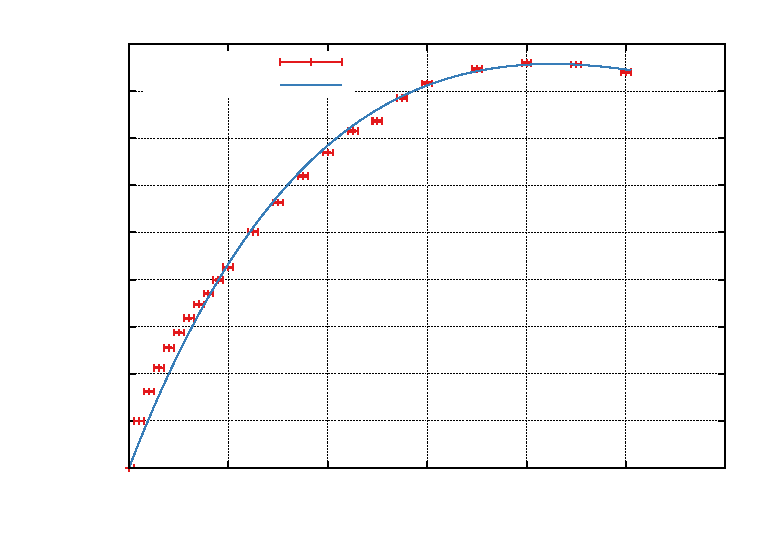
\includegraphics{./plots/totzeit}}%
    \gplfronttext
  \end{picture}%
\endgroup

	\caption{Abhängigkeit der Zählrate vom Emissionsstrom zur Abschätzung der Totzeit. Es handelt sich um ein paralysierendes System.}
\end{figure}
Es ist deutlich zu sehen, dass es sich bei dem beobachteten Aufbau um ein paralysierendes System handelt.
Dies ist erkennbar an der Tatsache, dass die Zählrate nicht wie für ein nicht-paralysierendes System erwartet in Sättigung geht, sondern nach Erreichen eines Maximums bei zunehmendem Emissionsstrom wieder abnimmt.

\subsection{Abschirmung}

\subsubsection{Korrigierte Zählraten}

\subsubsection{Transmissionen für Absorber}

\subsubsection{Transmissionskoeffizienten}

\subsection{Computertomographie}



\section{Fazit}

\FloatBarrier
% BIBLIOGRAPHIE
\vspace{\fill}
% Maximale Anzahl der Einträge in Klammer
% Zitieren mit \cite{lamport94}
\begin{thebibliography}{19}
\bibitem{siegbahn}
	K. Siegbahn,
	\emph{Alpha-, Beta- and Gamma-Ray Spectroscopy},
	Elsevier Science Ltd. 1965

\bibitem{anleitung}
	Physikalisches Praktikum V: Kern- und Teilchenphysik,
	Versuchsbeschreibung \emph{P523: $\beta$-Spektrometer} (Stand: Januar 2015),
	Universität Bonn	

\bibitem{riezler}
	Riezler, W.; Kopitzki, K.
	\emph{Kernphysikalisches Praktikum},
	Teubner 1963

\bibitem{nist}
	M. P. Unterweger, D. D. Hoppes, F. J. Schima, J.S. Coursey,
	\emph{NIST Radionuclide Half-Life Measurements},
	\url{http://www.nist.gov/pml/data/halflife-html.cfm} (Letzter Abruf: 1. Mai 2015)

\end{thebibliography}

% APPENDIX
\begin{appendix}
\section{Anhang}

\subsection{Abhängigkeit von Ionisationsstrom von der Kondensatorspannung}
\begin{table}[hp]
	\centering
	\begin{tabular}{SSSSSS}
	\toprule
	{$U_\mathrm{C}/\si{V}$} & {$\Delta U_\mathrm{C}/\si{V}$} & {$U_{I_\mathrm{C}}/\si{mV}$} & {$\Delta U_{I_\mathrm{C}}/\si{mV}$} & {$I_\mathrm{C}/\si{nA}$} & {$\Delta I_\mathrm{C}/\si{nA}$} \\ \midrule
	0.0      & 0.1         & 35        & 5            & 0.035     & 0.006        \\
	5.2      & 0.1         & 115       & 5            & 0.115     & 0.006        \\
	9.7      & 0.1         & 180       & 5            & 0.180     & 0.006        \\
	14.7     & 0.1         & 245       & 5            & 0.245     & 0.006        \\
	19.4     & 0.1         & 290       & 10           & 0.290     & 0.011        \\
	29.7     & 0.1         & 340       & 10           & 0.340     & 0.011        \\
	40.0     & 0.1         & 360       & 10           & 0.360     & 0.011        \\
	49.2     & 0.1         & 390       & 10           & 0.390     & 0.011        \\
	59.0     & 0.1         & 390       & 10           & 0.390     & 0.011        \\
	69.8     & 0.1         & 390       & 10           & 0.390     & 0.011        \\
	80.7     & 0.1         & 395       & 10           & 0.395     & 0.011        \\
	90.3     & 0.1         & 390       & 10           & 0.390     & 0.011        \\
	100.4    & 0.1         & 390       & 10           & 0.390     & 0.011        \\
	119.8    & 0.1         & 380       & 10           & 0.380     & 0.011        \\
	140.4    & 0.1         & 370       & 10           & 0.370     & 0.011        \\
	160.1    & 0.1         & 350       & 10           & 0.350     & 0.011        \\
	179.8    & 0.1         & 340       & 10           & 0.340     & 0.011        \\
	200.3    & 0.1         & 330       & 10           & 0.330     & 0.011        \\
	225.0    & 0.1         & 320       & 10           & 0.320     & 0.011        \\
	250.0    & 0.1         & 310       & 10           & 0.310     & 0.011        \\
	276.1    & 0.1         & 310       & 10           & 0.310     & 0.011        \\
	299.2    & 0.1         & 305       & 10           & 0.305     & 0.011        \\
	325.5    & 0.1         & 305       & 5            & 0.305     & 0.006        \\
	349.6    & 0.1         & 305       & 5            & 0.305     & 0.006        \\
	372.2    & 0.1         & 305       & 5            & 0.305     & 0.006        \\ \bottomrule
\end{tabular}
	\label{tab:kondensatorspannung_15kV}
	\caption{15kV}
\end{table}
\begin{table}[hp]
	\centering
	\begin{tabular}{SSSSSS}
	\toprule
	{$U_\mathrm{C}/\si{V}$} & {$\Delta U_\mathrm{C}/\si{V}$} & {$U_{I_\mathrm{C}}/\si{mV}$} & {$\Delta U_{I_\mathrm{C}}/\si{mV}$} & {$I_\mathrm{C}/\si{nA}$} & {$\Delta I_\mathrm{C}/\si{nA}$} \\ \midrule
	0.0   & 0.1 & 30   & 5  & 0.030 & 0.006 \\
	5.7   & 0.1 & 240  & 10 & 0.240 & 0.011 \\
	10.1  & 0.1 & 410  & 10 & 0.410 & 0.011 \\
	15.0  & 0.1 & 600  & 10 & 0.600 & 0.012 \\
	19.8  & 0.1 & 810  & 10 & 0.810 & 0.013 \\
	25.5  & 0.1 & 1050 & 20 & 1.050 & 0.023 \\
	30.3  & 0.1 & 1230 & 20 & 1.230 & 0.024 \\
	34.1  & 0.1 & 1360 & 20 & 1.360 & 0.025 \\
	40.4  & 0.1 & 1580 & 20 & 1.580 & 0.026 \\
	45.4  & 0.1 & 1690 & 20 & 1.690 & 0.027 \\
	49.1  & 0.1 & 1770 & 20 & 1.770 & 0.027 \\
	59.5  & 0.1 & 1920 & 20 & 1.920 & 0.028 \\
	70.3  & 0.1 & 1980 & 20 & 1.980 & 0.029 \\
	81.3  & 0.1 & 2060 & 20 & 2.060 & 0.029 \\
	89.4  & 0.1 & 2090 & 20 & 2.090 & 0.029 \\
	101.0 & 0.1 & 2110 & 20 & 2.110 & 0.030 \\
	120.2 & 0.1 & 2130 & 20 & 2.130 & 0.030 \\
	141.6 & 0.1 & 2130 & 10 & 2.130 & 0.024 \\
	159.9 & 0.1 & 2140 & 10 & 2.140 & 0.024 \\
	179.5 & 0.1 & 2115 & 10 & 2.115 & 0.024 \\
	200.3 & 0.1 & 2110 & 10 & 2.110 & 0.024 \\
	226.0 & 0.1 & 2070 & 10 & 2.070 & 0.023 \\
	251.2 & 0.1 & 2030 & 10 & 2.030 & 0.023 \\
	276.1 & 0.1 & 2010 & 10 & 2.010 & 0.023 \\
	300.2 & 0.1 & 2020 & 10 & 2.020 & 0.023 \\
	325.3 & 0.1 & 2000 & 10 & 2.000 & 0.023 \\
	351.3 & 0.1 & 1990 & 10 & 1.990 & 0.023 \\
	371.5 & 0.1 & 1990 & 10 & 1.990 & 0.023 \\ \bottomrule
\end{tabular}
	\label{tab:kondensatorspannung_25kV}
	\caption{25kV}
\end{table}
\begin{table}[hp]
	\centering
	\begin{tabular}{SSSSSS}
	\toprule
	{$U_\mathrm{C}/\si{V}$} & {$\Delta U_\mathrm{C}/\si{V}$} & {$U_{I_\mathrm{C}}/\si{mV}$} & {$\Delta U_{I_\mathrm{C}}/\si{mV}$} & {$I_\mathrm{C}/\si{nA}$} & {$\Delta I_\mathrm{C}/\si{nA}$} \\ \midrule
	0.0   & 0.1 & 30   & 10 & 0.030 & 0.011 \\
	5.2   & 0.1 & 300  & 20 & 0.300 & 0.021 \\
	9.5   & 0.1 & 550  & 20 & 0.550 & 0.021 \\
	14.2  & 0.1 & 810  & 10 & 0.810 & 0.013 \\
	19.9  & 0.1 & 1160 & 10 & 1.160 & 0.016 \\
	24.8  & 0.1 & 1480 & 10 & 1.480 & 0.018 \\
	29.2  & 0.1 & 1760 & 10 & 1.760 & 0.021 \\
	35.9  & 0.1 & 2180 & 10 & 2.180 & 0.024 \\
	40.5  & 0.1 & 2490 & 10 & 2.490 & 0.027 \\
	44.6  & 0.1 & 2730 & 10 & 2.730 & 0.030 \\
	49.1  & 0.1 & 3020 & 10 & 3.020 & 0.032 \\
	60.6  & 0.1 & 3640 & 10 & 3.640 & 0.038 \\
	68.8  & 0.1 & 3960 & 20 & 3.960 & 0.045 \\
	80.4  & 0.1 & 4330 & 20 & 4.330 & 0.048 \\
	89.0  & 0.1 & 4480 & 20 & 4.480 & 0.050 \\
	100.9 & 0.1 & 4680 & 20 & 4.680 & 0.051 \\
	119.0 & 0.1 & 4820 & 20 & 4.820 & 0.053 \\
	139.7 & 0.1 & 4970 & 20 & 4.970 & 0.054 \\
	159.9 & 0.1 & 5000 & 20 & 5.000 & 0.054 \\
	182.9 & 0.1 & 5000 & 20 & 5.000 & 0.054 \\
	202.0 & 0.1 & 5020 & 20 & 5.020 & 0.055 \\
	218.3 & 0.1 & 5050 & 50 & 5.050 & 0.072 \\
	243.7 & 0.1 & 5020 & 50 & 5.020 & 0.071 \\
	261.1 & 0.1 & 5000 & 50 & 5.000 & 0.071 \\
	280.0 & 0.1 & 4990 & 20 & 4.990 & 0.054 \\
	300.5 & 0.1 & 4980 & 20 & 4.980 & 0.054 \\
	326.0 & 0.1 & 4970 & 20 & 4.970 & 0.054 \\
	350.3 & 0.1 & 4950 & 20 & 4.950 & 0.054 \\
	374.6 & 0.1 & 4930 & 20 & 4.930 & 0.054 \\ \bottomrule
\end{tabular}
	\label{tab:kondensatorspannung_35kV}
	\caption{35kV}
\end{table}

\end{appendix}

\end{document}
